%%%%%%%%%%%%%%%%%%%%%%%%%%%%%%%%%%%%%%%%%%%%%%%%%%%%%%%%%%%%
% Document settings
\documentclass{ACGSeminar}

%%%%%%%%%%%%%%%%%%%%%%%%%%%%%%%%%%%%%%%%%%%%%%%%%%%%%%%%%%%%
% Own Packages
\usepackage{listings}
\usepackage{fancyhdr}

%%%%%%%%%%%%%%%%%%%%%%%%%%%%%%%%%%%%%%%%%%%%%%%%%%%%%%%%%%%%
% Own Definitions
\newcommand{\comment}[1]{}

%%%%%%%%%%%%%%%%%%%%%%%%%%%%%%%%%%%%%%%%%%%%%%%%%%%%%%%%%%%%
% BibTex
\bibliography{references}

%%%%%%%%%%%%%%%%%%%%%%%%%%%%%
% Hyphenations here
%%%%%%%%%%%%%%%%%%%%%%%%%%%%%
\hyphenation{Sa-tan-arch-aeo-li-deal-co-hell-ish}

%%%%%%%%%%%%%%%%%%%%%%%%%%%%%
% Title, Author, etc.

\pagestyle{fancy}
\fancyhf{}
%\rhead{}
%\lhead{\leftmark \rightmark}
\fancyhead[R]{\nouppercase{\leftmark}}
\fancyhead[L]{\nouppercase{\rightmark}}
\fancyfoot[C]{\thepage}

\begin{document}

\title{Re: Deep G-Buffers for Stable Global Illumination Approximation}

\author{Ferit Tohidi Far}

\maketitle

%%%%%%%%%%%%%%%%%%%%%%%%%%%%%%%%%%%%%%%%%%%%%%%%%%%%%%%%%%%%
% Abstract

\begin{abstract}%
G-buffers can be used to efficiently render images with large amounts of light sources. This is possible thanks to a process called "deferred rendering". Using 
only g-buffers, we are only able to compute local illumination, which forces us to find a way to achieve sought after visual and lighting effects like global 
illumination. By using deep g-buffers we can approximate global illumination in a way that is more efficient than traditional methods like pathtracing, 
while of course not being physically accurate. We can make up for it, though, by also approximating visual effects like ambient occlusion, color bleeding, reflections, 
depth of field and motion blur to create an acceptable interactive realtime result, which is - as of now - simply impossible with physically accurate methods on 
average hardware.
\end{abstract}

\keywords{nvidia, g-buffer, deep g-buffer, pathtracing, global illumination approximation, deferred shading, deferred rendering}
\tableofcontents
\listoffigures
\listofalgorithms

\label{cha:references}

\newpage

%%%%%%%%%%%%%%%%%%%%%%%%%%%%%%%%%%%%%%%%%%%%%%%%%%%%%%%%%%%%
% Introduction
\label{cha:introduction}
\section{Global illumination}
	In order to understand why computing global illumination is such a big deal, we first need to set the stage by introducing the essentials of traditional rendering. \\\\
	Global illumination is a lighting effect that is achieved by not only computing direct light, but also indirect light, meaning that it is neccesary to take	into account how light reflects and carries information (in the most basic case: color). On the contrary, local illumination is computed by only considering direct light, meaning that the resulting image will lack details and visual effects that would otherwise convey realism. These visual effects are ambient occlusion, color bleeding, reflections, caustics, and soft shadows. What all these visual effects describe is explained in section 4.
	\subsection{Physically correct methods}
	In order to generate physically correct lighting, which is a requirement for creating photorealistic images, we need to solve the rendering equation
	$$ L_o(\omega) = L_e(\omega) + \int_\Omega f(\omega, \omega')L_i(\omega')cos(n, \omega') \partial \omega' $$
	where 
	\begin{center}
		\begin{align*}
			&L_o(\omega) \text{ is the outgoing light in direction } \omega\text{,}\\
			&L_e(\omega) \text{ is the emmited light in direction } \omega\text{,}\\
			&f(\omega, \omega') \text{ is the BRDF\footnotemark} \text{,}\\
			&L_i(\omega') \text{ is the incoming light from direction } \omega'\\
			&\text{and } cos(n, \omega') \text{ is lambert reflectance\footnotemark}  \text{ .}
		\end{align*}
	\end{center}
	\addtocounter{footnote}{-1}
	\footnotetext{The bidirectional random distribution function basically describes the reflection/refraction of a ray on surface.}%
	\stepcounter{footnote}
	\footnotetext{Lambert reflectance describes the attentuation of light on diffuse objects based on the lights incident angle.}%
	The most popular method for achieving this is pathtracing \cite{P2PATH}.
	\subsubsection{Pathtracing} 
		solves the rendering equation by first sending camera rays through each individual pixel of the image plane and then tracing the ray back to the light source. If the lamp is hit the pixel gets painted painted with color, else black. Direct consequences of this are soft shadows and ambient occlusion. A maximum hop number caps the amount of times a ray is able to reflect. A hop number larger than 1 (3 in most simple cases is sufficient, but it is dependent on the complexity of the scene) allows for global illumination. The reflections and refractions are essentially determined by the BRDF, which not only means that objects can be transparent, but we also get caustics\footnote{Caustics are areas with concentrated light. This happens due to light refracting.}. With each sxurface a ray hits it carries information from that surface, e.g. its color, and reflects it onto the next surface it hits. This causes color bleeding. Each pixel is sampled thousands - possibly hundreds of thousands - of times to reduce the noise that is induced by diffuse reflections, resulting in a photorealistic render.
		\begin{figure}[htb!]%
			\begin{center}%
				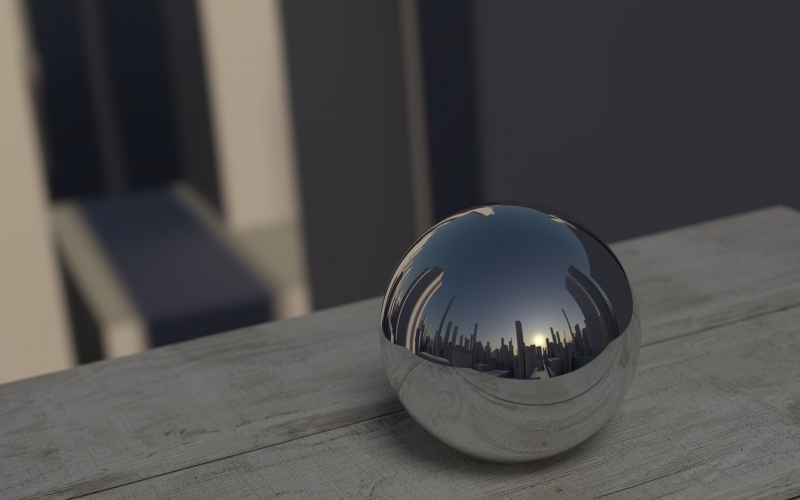
\includegraphics[width=7cm]{img/pathtracing.png}
			\end{center}%
			\caption{A photorealistic computer generated image using pathtracing.}%
			\label{fig:pathtracing}%
		\end{figure}%
	\subsubsection{Radiosity}
		is a diffuse global illumination method, meaning it is only meant to be used for diffuse surfaces, as it is has been observed to be one of their physical properties. In simple terms, it solves the rendering equation by splitting the objects in cameraspace into patches and treats each of those as a light emitter. We iteratively check which patches are exposed to light (an initial light-source is required) and adjust their emmitances accordingly until convergence or until we are satisfied with the look of the render (see figure \ref{fig:radiosity}). It takes a while to compute the illumination, but since it is not dependent on the camera view or location, the illumination can will stay the same unless an object is moved. Games often preprocess radiosity on scenes with little object movement as it then becomes a quick way of achieving diffuse global illumination \cite{RAD}.
		\begin{figure}[htb!]%
			\begin{center}%
				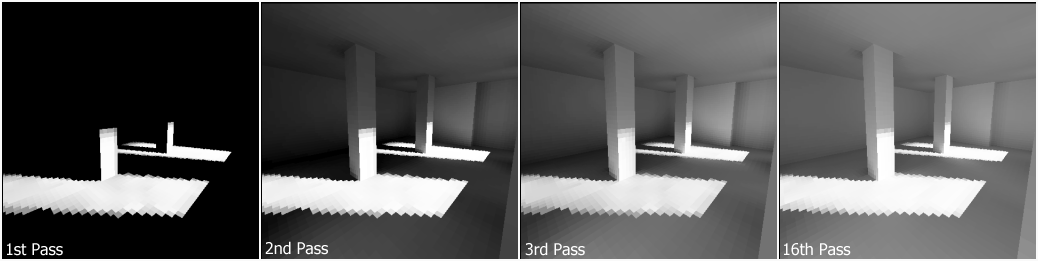
\includegraphics[width=16cm]{img/radiosity.png}
			\end{center}%
			\caption{How radiosity globally illuminates a scene. With each iteration there are more light emitters, meaning that there are more possible patches that can be illuminated. In the first iteration, the only light-emitters are the windows (not visible in the frame). After 16 iterations the scene is sufficiently saturated.}%
			\label{fig:radiosity}%
		\end{figure}%
	\subsection{Computational difficulties of physically correct methods}
	With pathtracing we have to take into account thousands of samples of every ray of light with its reflections, so the computational difficulty should become apparent \cite{DST}. Radiosity can be preprocessed and quickly loaded to illuminate a scene, but thus would require large amounts of memory for non-static scenes. Because of this, it is nearly impossible to achieve real time rendering using physically correct methods on an average system. This forces game engines to stick to \textbf{faking} global illumination and visual effects since it is way more efficient to compute. Adding multiple light sources to the scene will still be challenging to average systems with traditional rendering (forward rendering) as described by modern graphics pipelines. Deferred rendering, specifically deferred shading, counters this problem at the cost of having to compute transparency using depth peeling and having no straight forward anti-aliasing\footnote{Anti-aliasing is a method that tries to smoothen out pixelated-looking edges.}.

\section{Deferred rendering}
	Graphics pipelines describe each step that has to be taken in order to render an image. Within a pipeline it is possible in some cases to defer steps to a later stage. It is conventional to use GPU's for applications that rely heavily on rendering images. There is no universal graphics pipeline, because these are dependent on the GPU that is used, which means it is convenient that there exist API's like OpenGL that try to generalize the steps that need to be taken in order to render an image and map them to compatible GPU's. This means that most GPU dependent applications abide by the graphics pipeline as described by, for instance, OpenGL (figure \ref{fig:graphics_pipeline}).
	\begin{figure}[htb!]%
	\begin{center}%
		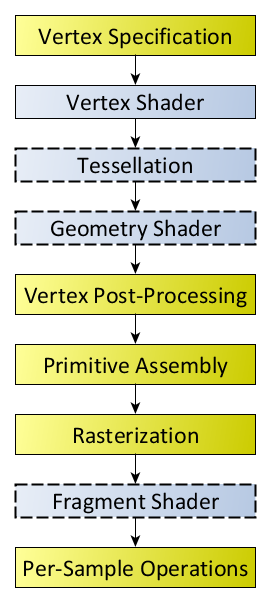
\includegraphics[height=7cm]{img/graphics_pipeline.png}
	\end{center}%
	\caption{The OpenGL graphics pipeline. All steps are mandatory, but the ones within blue boxes are also programmable and the ones with dashed borders can be deferred or forwarded. Note that the vertex-shader and geometry-shader do not neccesarily compute any shading or colors, but can be programmed to do so. They are called shaders for historical reasons, which might be a little irritating.}%
	\label{fig:graphics_pipeline}%
	\end{figure}%
	\subsection{How deferred shading handles lighting more efficiently}
		The goal of deferred shading is to defer the shading stage. Instead of shading right away, we compute necessary geometry buffers (g-buffers) in a first pass that we call "geometry pass" and cache 
		them for later use in the second pass which we call "shading (or lighting) pass". \\\\
		With forward rendering we would have to compute the shading for every fragment of every object for all light-sources in a single pass. The shading is applied regardless wether the fragment is visible at the end or not, since the visibility test is performed at the end. This means that the time complexity of computing forward shading is $O(amount_{fragments} \cdot amount_{lights})$. \\\\
		If we apply deffered shading, however, we do not force ourselves to shade every fragment as soon as it has been computed, instead we wait until we find the closest fragment so to say. Finding the closest fragment is called "solving the visibility problem". This is solved during the geometry pass when filling the z-buffer with its respective z-values, which can be computed by performing perspective correct interpolation between the vertices of the current polygon (in most cases triangles). The z-buffer, along with all other buffers that are collected, are continuously updated if a closer fragment for the same pixel is found, which solves the visibility problem. Now all the fragments that we shade are only going to be shaded once, which means for the time complexity that the shading is done in $O(amount_{pixels} \cdot amount_{lights})$, allowing us to render more light-sources at the expense of passing around g-buffers (note that fragments are \textbf{potential} pixels). \\\\
		For all practical purposes, g-buffers have to at least consist of a frame-buffer, a normal-buffer and a z-buffer. Using only these g-buffers, it is possible to render an image with basic shading.

		\begin{figure}[htb!]%
		\begin{center}%
			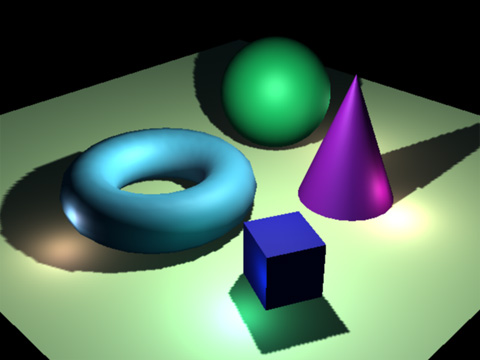
\includegraphics[width=7cm]{img/wiki_deferred_shading.png}
		\end{center}%
		\caption{A scene that was rendered using deferred shading. The objects are locally illuminated by point-lights using g-buffers.}%
		\label{fig:deferred_shading}%
		\end{figure}%

\section{Geometry-buffer (g-buffer)}
	Each geometry-buffer stores information of some sort for each individual pixel, meaning that they are all two-dimensional arrays using the dimensions of the screen. Note that there are more possible buffers to choose from, but the three that will be mentioned are the most essential in every g-buffer.
	\subsection{Frame-buffer}%
		Color-values of fragments are stored in the frame-buffer. It basically stores the rendered image without fragment-shading\footnote{Fragment-shading (also called pixel-shading) aims to shade every single fragment by using some shading technique.} applied to it.% 
		\begin{figure}[htb!]%
			\begin{center}%
				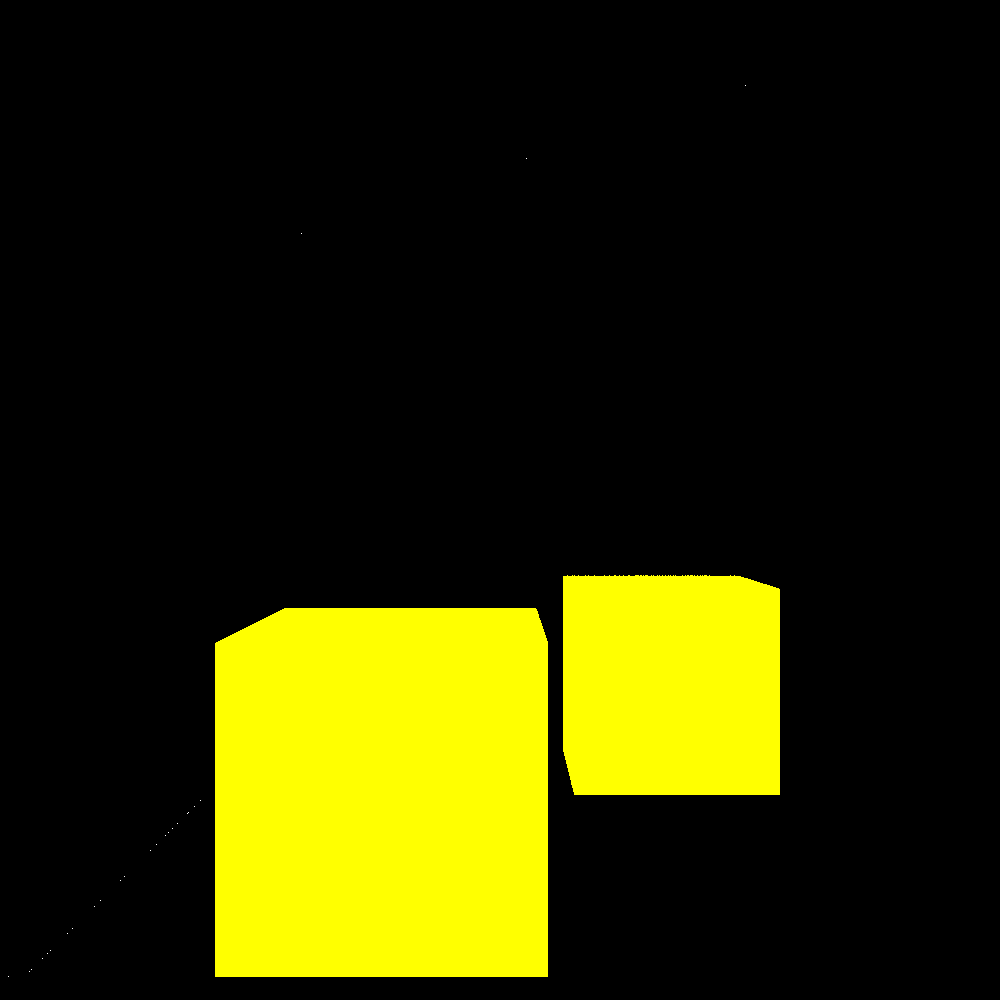
\includegraphics[width=7cm]{img/frame_buffer.png}
			\end{center}%
			\caption{Example of a frame-buffer (also called image-buffer). It shows a cornell box with pitch black walls containing two yellow cuboids.}%
			\label{fig:frame_buffer}
		\end{figure}%
	\subsection{Z-buffer}
		The z-buffer stores depth values of fragments. These are needed to determine which surfaces are closest and visible to the camera. If two different fragments\footnote{A fragment is a point on a surface in worldspace\footnotemark} have the same x and y coordinates in screenspace\footnotemark, then the fragment with the smaller z-value is supposed to be in front of the other. This buffer is also used for screenspace visual effects like screen space ambient occlusion and depth peeling. 
		\addtocounter{footnote}{-1}
		\footnotetext{Worldspace is the space in which the 3d objects are placed.}
		\stepcounter{footnote}
		\footnotetext{Screenspace is the space in which the individual pixels of the projected 3d models are defined.}
		\begin{figure}[htb!]%
			\begin{center}%
				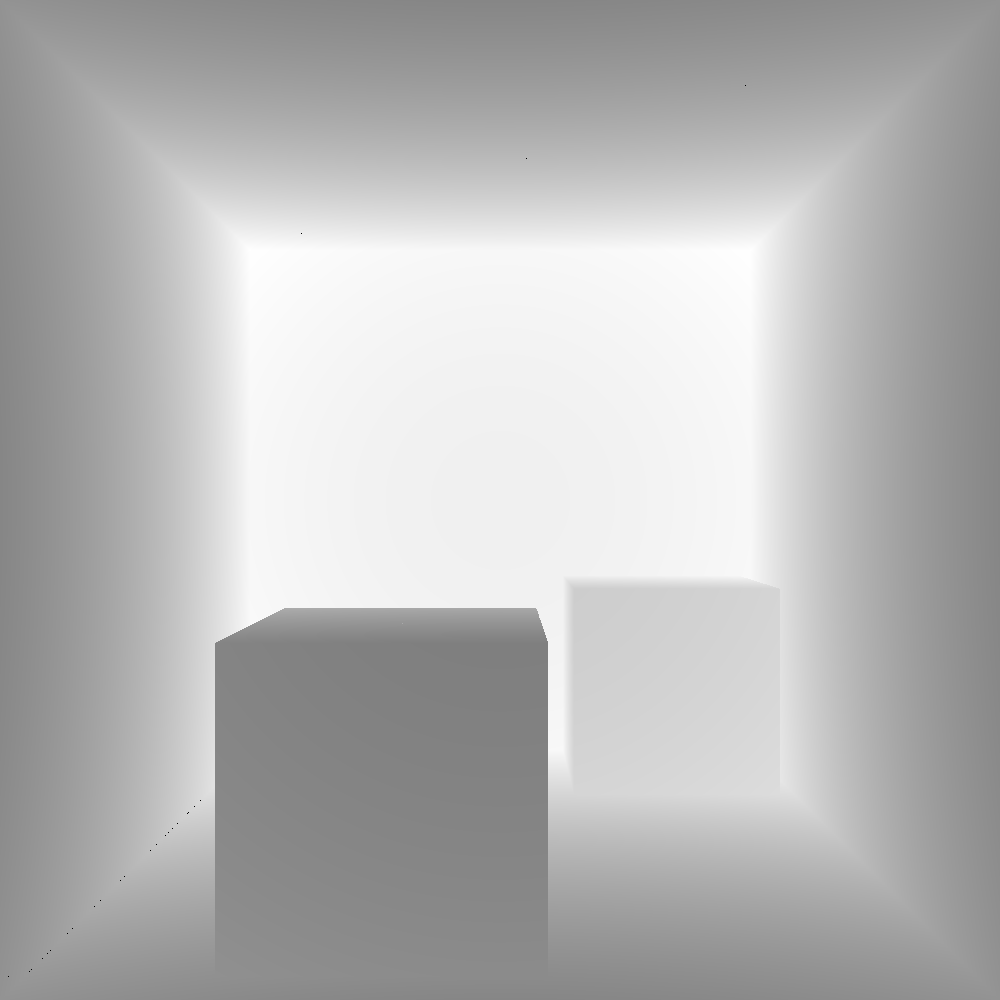
\includegraphics[width=7cm]{img/z_buffer.png}
			\end{center}%
			\caption{Example of a z-buffer. Since the z-buffer only stores distances as float values deduced by dividing each
			z-value by the distance of the furthest away object from the cameras point of view, which is the maximum z-value, they are interpreted as a grayscale value which is turned into an RGB vector by multiplying $(z, z, z)$ with $255$.}%
			\label{fig:z_buffer}
		\end{figure}%
	\subsection{Normal-buffer}
		The normal-buffer stores surface-normals that are mostly used for shading and to determine reflection and refraction directions. They can also be used for light attentuation, since the dot product of a normalized surface-normal and the normalized direction of a light-ray is a criterion for light intensity. If the light-ray is orthogonal to the surface-normal, for instance, the dot product will equal zero, meaning that the light has maximum intensity (lambert reflectance).
		\begin{figure}[htb!]%
			\begin{center}%
				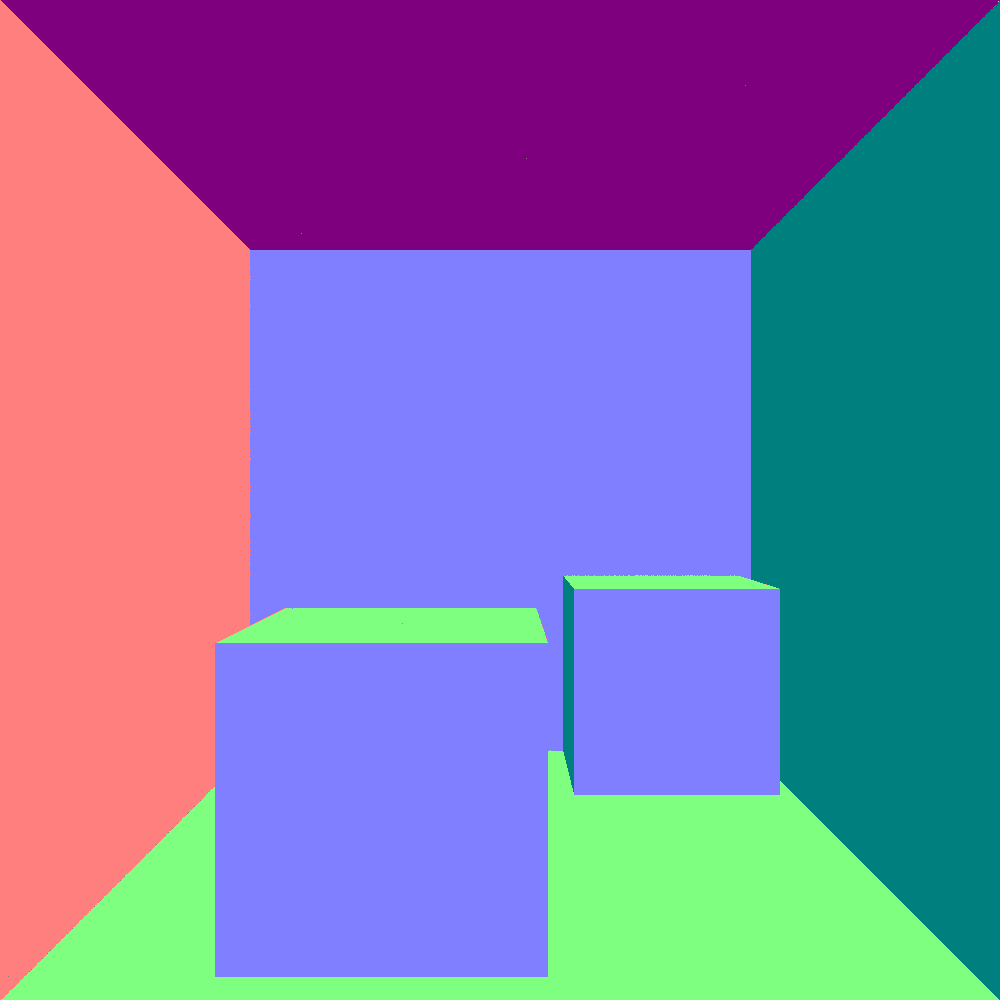
\includegraphics[width=7cm]{img/normal_buffer.png}
			\end{center}%
			\caption{Example of a normal-buffer. Normal vectors in this buffer are normalized, meaning their component values range from -1 to 1. Since negative normals would cause negative RGB values, we add $(1, 1, 1)$ and scale with $255/2$, which results in a usable RGB color.}%
			\label{fig:normal_buffer}
		\end{figure}%
	\subsection{Computing local illumination using g-buffers (deferred shading)}
		For any illumination to happen we first need to define some light sources. The following are some of the possible light-sources that we can use:
		Point-lights, spot-lights and directional-lights \cite{DST}. The simplest one is directional-light. We simply specify an origin in worldspace from which the light rays are sent in all directions. A point-light is a directional-light which is constrained by its radius (basically a sphere of light). Finally, spot-lights are area lights which emit light on another area (like spot-lights in real life do). 
		%TODO fix explanation on light sources a little
		At this point we have to choose a shading technique. The most popular ones are gouraud-shading and phong-shading. \\\\
		Both first compute the normals for each vertex for each polygon in cameraspace within the vertex-shader. This can be done by averaging the surface normals of the polygons that share the vertex of which the normal is to be computed. The differences are essentially that gouraud-shading computes shaded colors using some illumination-model\footnote{An illumination-model is a way of describing how a light-source effects the color of a fragment that it hits. This will vary depending on the light-source that is used.}, which requires vertex-normals that were just computed, and assigns them to the vertices of their polygons within the vertex-shader and then interpolates (blends) the fragment-colors inbetween the vertices in the fragment-shader, while phong-shading uses its vertex-normals to interpolate the normals of each fragment within the polygons in the vertex-shader and computes shaded colors using some illumination-model, which requires the fragment-normals that were just computed, on each fragment in the fragment-shader. \\\\
		Gouraud-shading is a fast way of computing shading since it only uses the illumination-model on each vertex of its polygons (which would be three times if the polygons are triangles) as opposed to applying the illumination-model on each fragment, as well as computing the normal for each fragment, as is done by phong-shading. On the downside, gouraud-shading may look edgy if the 3d models are made of few polygons, which would make phong-shading preferable in that case. This would conclude local illumination, which means we took care of direct lighting. \\\\
		In the context of deferred shading, all of this is done in the second pass (the shading or lighting pass). By now it should become apparent why shading in a single pass is inefficient, since all of these illumination computations would be in vein if the visibility test does not pass anyway. The g-buffers that we collect in the first pass (the geometry pass) make this possible. 

\section{Visual effects} 
	The following are visual effects that are sought after, but some of them are hard or impossible to achieve physically correct without using
	computationally expensive methods. When applying pathtracing, we get most of the following effects for free: 
	\begin{figure}[htb!]%
	\begin{center}%
		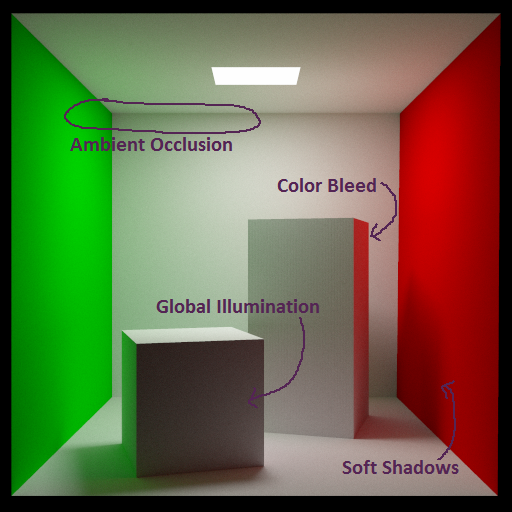
\includegraphics[width=7cm]{img/visual_effects.png}
	\end{center}%
	\caption{Diverse visual effects caused by global illumination inside a cornell box. The image was rendered using pathtracing.}%
	%TODO insert source https://blog.demofox.org/2016/09/21/path-tracing-getting-started-with-diffuse-and-emissive/
	\label{fig:visual_effects}%
	\end{figure}%
	\subsection{Ambient occlusion}
		Ambient occlusion essentially describes how much shading the "in-betweens" of a 3d object gets \cite{AOM}. This effect can be efficiently approximated by using a method called - ironically - screen space ambient occlusion (SSAO). \\\\
		This method basically checks the surrounding z-values of each z-value of the z-buffer. Given a radius $r$ and a sampling count $N$ we can compute the ambient occlusion factor $AO$ by checking $N$ randomly picked surrounding z-values within $r$. In simple terms, if the majority (half or more) of the samples (the surrounding z-values) are smaller than the center z-value (the one we are computing $AO$ for), then $AO$ receives a value of $1$, else a value smaller than $1$ but larger or equal to $0$. These float values can then be put in a texture-buffer to be used in post-processing or they can be used directly. To apply ambient occlusion to the final image, the $AO$ values are multiplied with their respective pixels in the final image. Because $0 \leq AO \leq 1$ this can be seen as tweaking the intensity of the color on a specific pixel. \\\\
		Since it only runs over the z-buffer it is considered screen space. Ambient occlusion (the visual effect) is an effect directly caused by global illumination, leading the method (ambient occlusion) to be considered an efficient way of faking global illumination.
		\begin{figure}[htb!]%
			\begin{center}%
				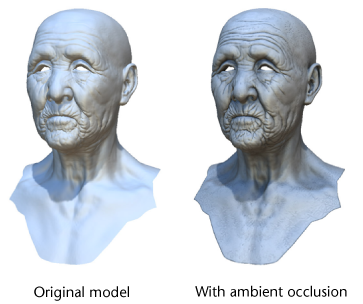
\includegraphics[width=7cm]{img/ambient_occlusion.png}
			\end{center}%
			\caption{How ambient occlusion affects the realism of a rendered 3d model. The "in-betweens" of the model appear to have depth.}%
			\label{fig:ambient_occlusion}%
		\end{figure}%
	\subsection{Color bleeding}
		Color bleeding happens when light directs information from one hit-surface to another. Let A and B be objects. If A reflects light onto B and A's surface is blue, then B will also appear
		to be slightly blue on the reflected area. To have this happen it would obviously be convenient to trace rays of some sort. Point-based color bleeding approximates this by using point cloud surfels with direct illumination values \cite{PBCB}. As this is somewhat complicated to put into few phrases, we recommend reading the paper "Point-Based Approximate Color Bleeding". On the other hand, we will be presenting a simpler method using deep g-buffers in section 5.

	\subsection{Soft shadows}
		We can easily compute hard shadows in screen space using shadow mapping. A shadow map is a buffer that contains the distances between the light source and all pixels (visible fragments) of the scene. Having created the shadow map we check if the entry in the z-buffer is larger than the entry in the shadow map. If so, then the fragment is in shadow and is painted black. If not, then the fragment keeps its color and we can proceed to compute its local illumination. This can be extended to soft shadows simply by blending together fragments in shadow with their surrounding fragments.

	\subsection{Transparency}
		A quick method to achieve transparency is depth peeling. To do this we need two g-buffers at a time, one of which stores the current g-buffer and one of which stores the previous g-buffer. Depending on how many levels of transparency are wished for, let $k$ be the level of transparency, we make $k$ passes on the g-buffers, "peeling" away the previous g-buffers texel\footnote{A texel is essentially a pixel of a texture. G-buffers are stored in texture-buffers inside the GPU, which means their individual pixels can be refered to as texel.} from the current g-buffer if a larger z-value on that texel-position is found. For this to work, the previous z-buffer in the first pass has to be initialized with negative infinity \cite{NOIT}.
		%TODO explain how to construct the final transparent image

	\subsection{Reflection}
		Screen space reflections can be efficiently computed. If the reflective surface is completely planar, then we can simply project the texture that is supposed to be reflected onto the surface that reflects it. \\\\
		In all other cases, we rely on cube mapping (also called environmental mapping or reflection mapping). Creating a cube-map (figure \ref{fig:cube_map}) works like this: we define a cube with our camera in its inner center. Next, we treat each plane of the cube as an image plane that we render to, meaning we render six times in total, and save those inside a buffer. This buffer now has knowledge about the entire surrounding environment of the reflective object. When computing the color of a vertex of a reflective object, we use the direction vector from the camera to the vertex and use the vertex-normal to get the specular reflection direction, which will ultimately point at the spot on the cube-map that will be reflected. The issue with this is that it lacks the ability to self-reflect \cite{REFL}.
		\begin{figure}[htb!]%
			\begin{center}%
				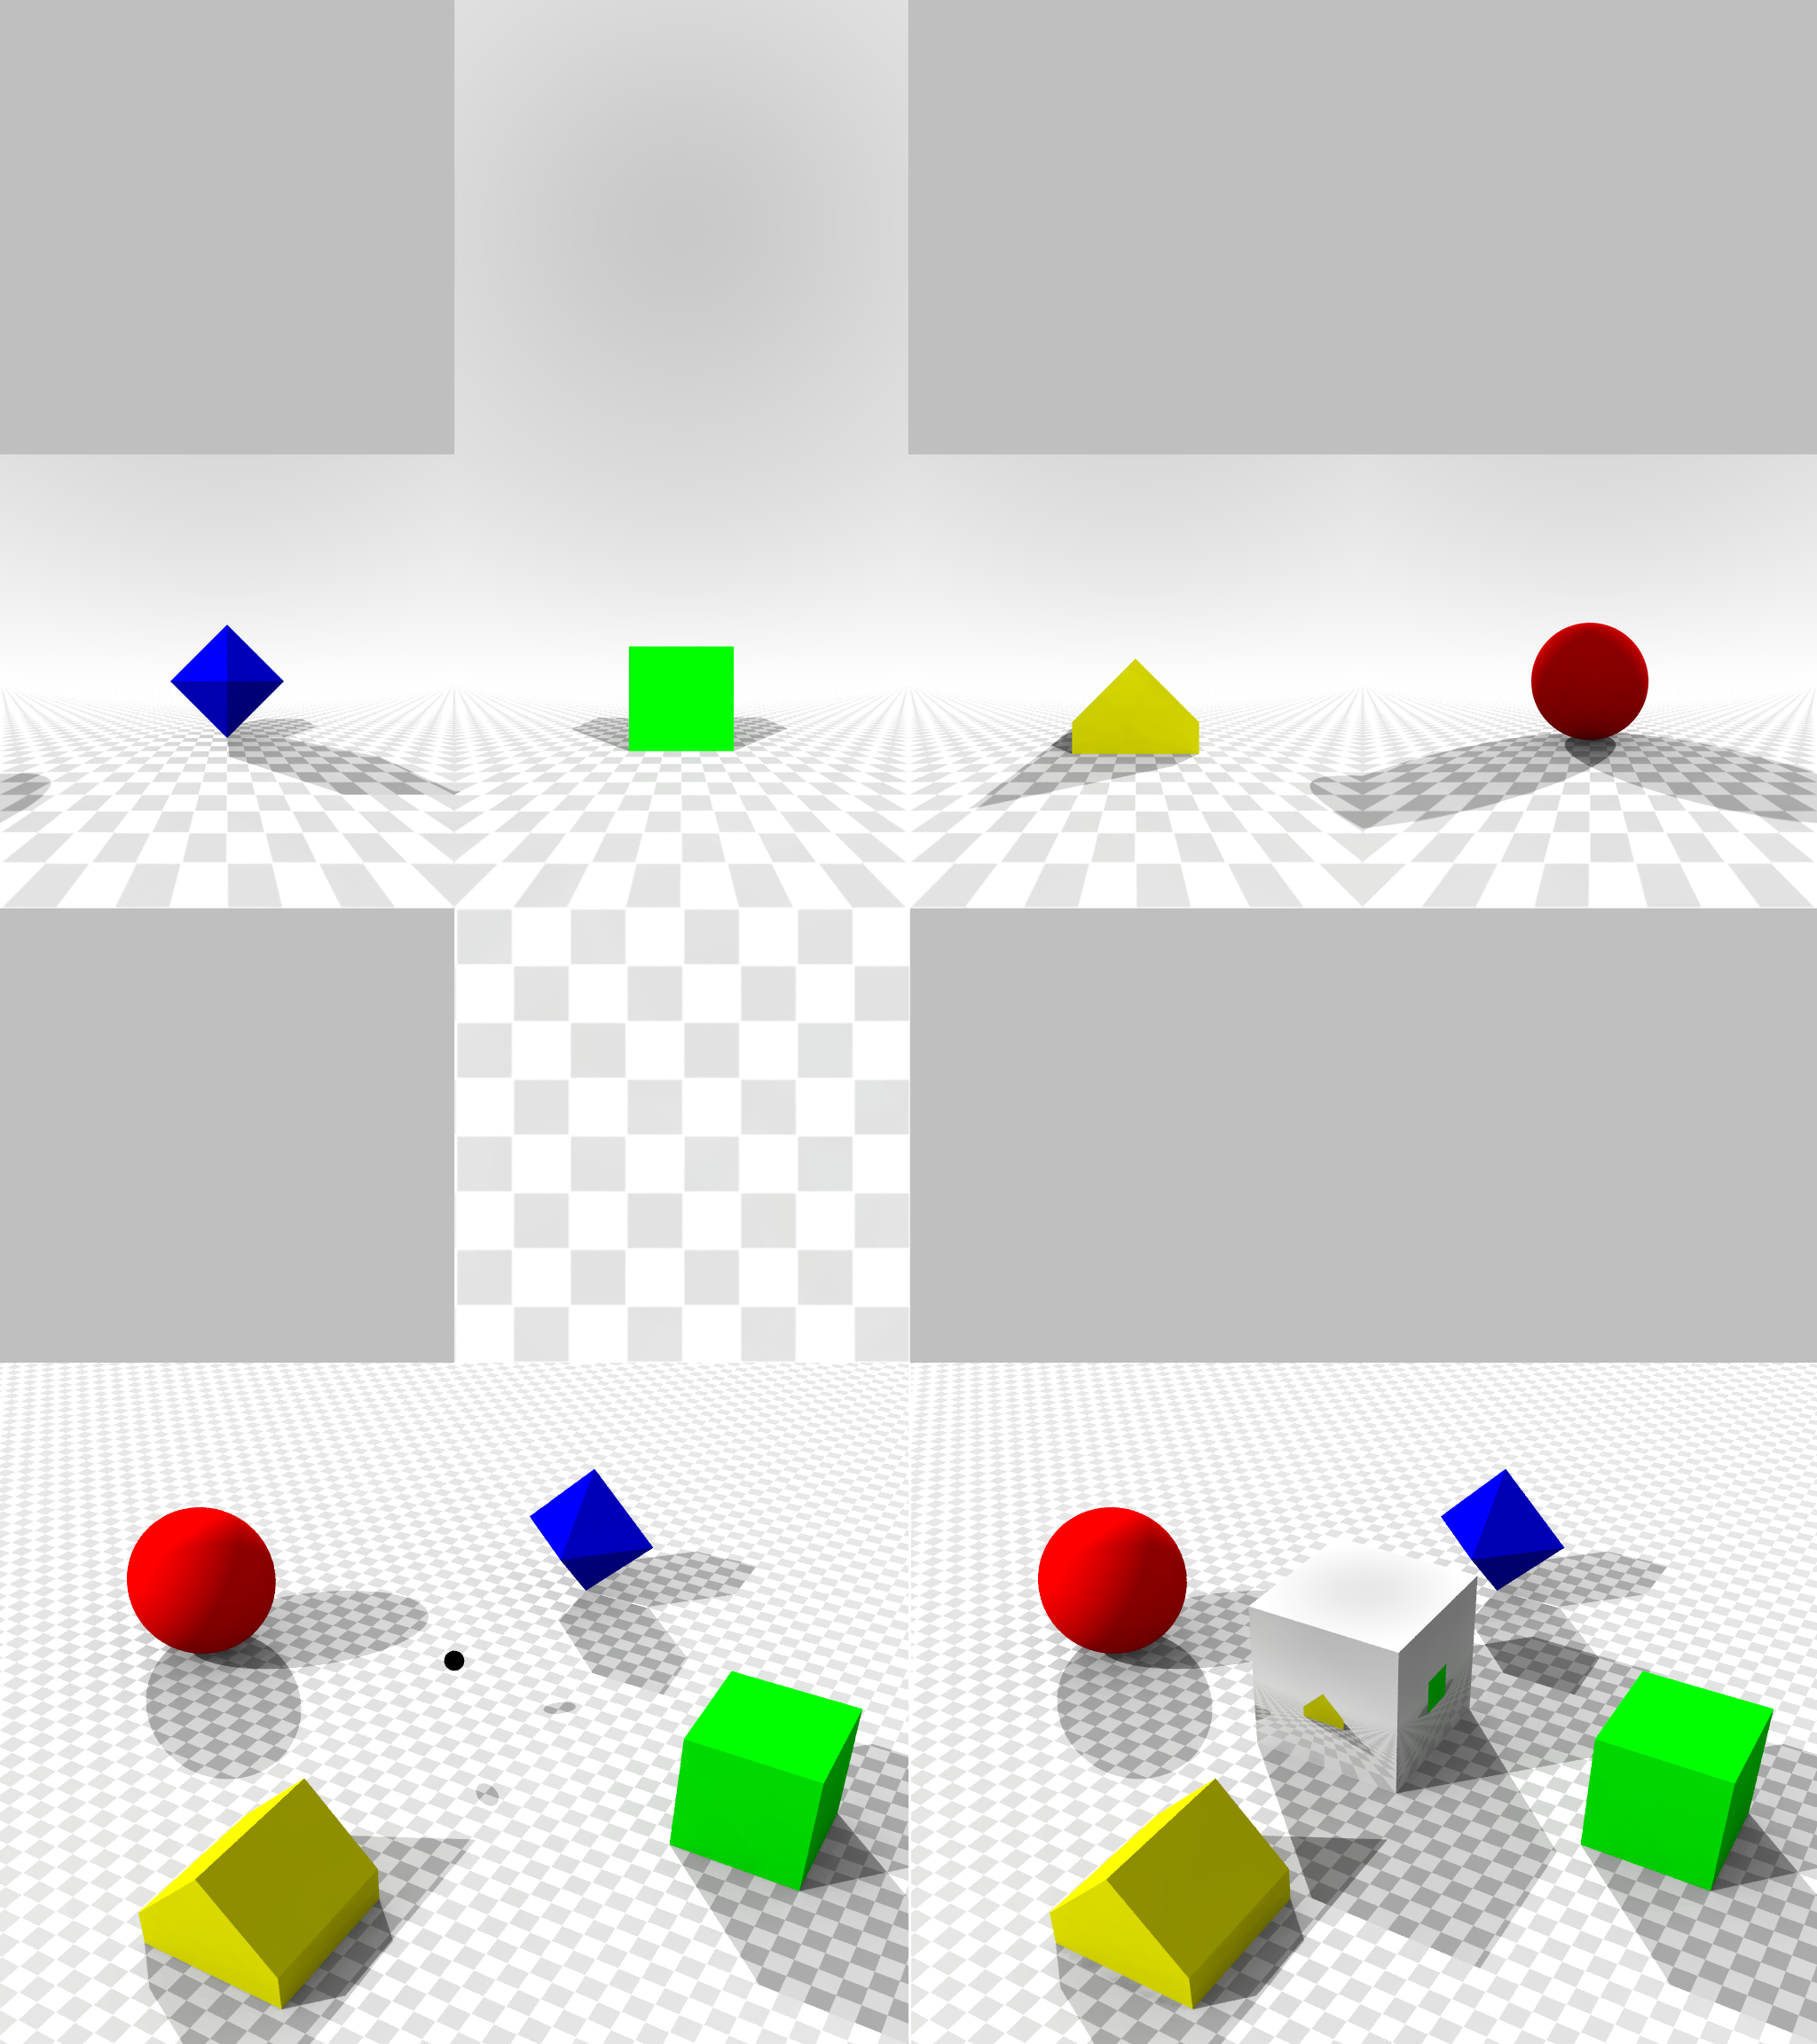
\includegraphics[width=7cm]{img/cube_map.png}
			\end{center}%
			\caption{How a cube-map is rendered. The black sphere in the lower image represents the camera. The resulting six renders are put together in the cube-map in the upper image.}%
			\label{fig:cube_map}%
		\end{figure}%

	\subsection{Depth of field}
		Depth of field is an effect that arises when the lens of a camera is larger than just a pinhole. This allows for more light to pass through the lens and light-rays start to intersect each other, causing the resulting image to look blurry along certain distances. A raytracer could simply achieve this by sampling its camera rays over a circle. For a rasterizer it is much more complicated. This effect could be achieved using stochastic point samples along the lens in 4D \cite{DOF2}. As this is also difficult to briefly summarize, we recommend reading the paper "High-Quality Parallel Depth-of-Field Using Line Samples". 
		\begin{figure}[htb!]%
			\begin{center}%
				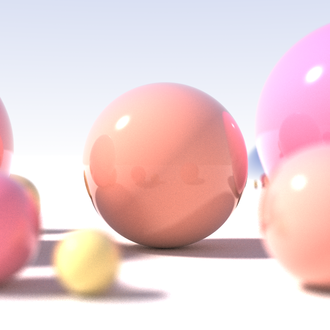
\includegraphics[width=7cm]{img/raytraced_depth_of_field.png}
			\end{center}%
			\caption{Depth of field in action. The camera lens is focused on the center sphere, making it appear sharp. The other spheres appear to be blurry.}%
			\label{fig:depth_of_field}%
		\end{figure}%

	\subsection{Motion blur}
		Motion blur is a camera effect that comes up when the camera or an object in the scene is moving while a picture is being taken. The camera requires itself and the objects in the scene to be still in order for light to hit the lens in focus. If the camera or an object is moving while the light is hitting the lens, then the light of the new scene will intersect the light of the old scene causing a blur. This effect can be easily rendered in screen space by taking into account in which direction the camera or the object is moving, as well as at what velocity, which can also be evaluated using the previous frame, and blurring accordingly \cite{MOB}.

\section{Deep g-buffer}
	Deep g-buffers make use of a concept similar to depth peeling. Instead of storing information about the closest surface, in an n-layer deep g-buffer we also store information about the n-closest surface \cite{Mara2016DeepGBuffer}. This means we store g-buffers for the closest surfaces, then the second-closest surfaces and eventually the n-closest surfaces in an n-layer deep g-buffer. \\\\
	Practical observations suggest that the second-closest surface is often not the second-most relevant for shading and visual effects \cite{Mara2016DeepGBuffer}. To resolve this issue we rely on minimum depth separation, which essentially introduces a distance $\Delta z$ that has to be exceeded when looking for the next-closest surface immediately after the current one. Setting $\Delta z = 0$ makes the generated 2-layer z-buffer of the deep g-buffer turn into a 2-layer k-buffer\footnote{A k-buffer is a k-layer z-buffer that stores the z-values of the k-closest polygons in order. Unlike with deep g-buffers, the minimum separation constraint is not met.} \cite{MFEKB}. \\\\
	How to pick $\Delta z$ ultimately depends on the depth complexity of the scene and has to be tweaked accordingly. If $\Delta z$ is too large, it is possible that important visual information might be missed. On the other hand, if $\Delta z$ is too small, it is possible that unnecessary information might be picked up. According to NVIDIA, $\Delta z = 50cm$ seems to consistently deliver stable results, at least in the renders done in their paper.
	\subsection{Generating a 2-layer deep g-buffer}
		NVIDIA proposes two ways of generating a 2-layer deep g-buffer, one of which is straight forward to help demonstrate the idea and one of which is efficient. \\\\
		The first one is called "Strawman Two-Pass Generation Algorithm" and displayed in algorithm \ref{alg:two_pass_strawman}. $Z$ is the 2-layer z-buffer, $S(x, y, z)$ returns other g-buffers needed for shading and $T(tri)$ applies the transformation $T$ to triangle $tri$ (model-view-projection\footnote{Each object has a model-view-matrix that describes at which location, at what which angle and at which size it has to appear in the scene.} and skinning-transformations\footnote{Skinning is a term from computer animation that assigns joints to an object that can move.}). In the first pass we simply collect the first layers g-buffers and in the second pass we peel away the first layers g-buffers to receive the second layer. Since fragments get discarded if their distance to the previous fragment is smaller than $\Delta z$ the minimum depth seperation constraint is met. \\\\
		This is essentially two-pass depth peeling, however, there is a more efficient algorithm which only requires a single pass displayed in \ref{alg:one_pass_strawman}. \\\\
		In order to save a pass over the geometry, we rely on an oracle that predicts the first layers z-buffer before it is even rendered. Using that prediction, we can compute fragments for the second layer by peeling the first layer. In total, there are four variants to go about this. $t$ is the index of the frame.
		\begin{enumerate}
			\item \textbf{DELAY VARIANT} manages to predict the first layers z-buffer by adding a frame of latency, meaning that what is happening in the scene (animations, object movements and such) and what is being rendered on the screen is out of sync by one frame. This way, the next frames transformation $T_{t+1}$ is known at render time, enabling us to predict first layer z-buffers perfectly (since we do not really predict it anyway). The downside to this is, obviously, the frame latency.

			\item \textbf{PREVIOUS VARIANT} approximates the first layer z-buffer by taking the previous frames first layer z-buffer. This will deliver good results if camera- and object-movement are minimal, but even then, the errors would appear in the second layer, which is not visible to begin with (excluding transparent objects). It does not guarantee minimum separation.

			\item \textbf{PREDICT VARIANT} uses velocities from the underlying physics simulation or animation to predict the next transformation $T_{t+1}$. Alternatively, extrapolation over the change in vertices from the previous and current frame would also work. Accurate velocity prediction will deliver accurate results without latency. In the other case, drawbacks are equivalent to that of the \textit{PREVIOUS VARIANT}

			\item \textbf{REPROJECT VARIANT} performs the minimum separation test against the first layer z-buffer of the previous frame. The visibility test is done using screen coordinates and z-values computed using the vertices of the previous frame, meaning the visibility test is done in the "past". Like with \textit{PREDICT VARIANT}, moving objects are a source of error, but the velocities computed in this case are perfect, which means the errors are not as bad. Benchmarks suggest that compared to all the other variants, this delivers the most stable performance at the greatest speed.

		\end{enumerate} 
		\begin{algorithm} \label{alg:two_pass_strawman} \caption{Strawman two-pass generation algorithm for generating 2-layer deep g-buffers}
		\begin{lstlisting}[frame=single]
//1st pass
submit geometry with:
  geometryShader(tri):
    emit T(tri) to layer 0
  pixelShader(x, y, z):
    return S(x, y, z)

//2nd pass
submit geometry with:
geometryShader(tri):
    emit T(tri) to layer 1
  pixelShader(x, y, z):
    if z > Z[0][x][y] + \Delta z:
      return S(x, y, z)
    else:
      discard fragment
		\end{lstlisting}
		\end{algorithm}
		 
		\begin{algorithm} \label{alg:one_pass_strawman} \caption{An improved one-pass algorithm for generating 2-layer deep g-buffers}
		\begin{lstlisting}[frame=single]
submit geometry with:
  geometryShader(tri)
    emit T(t, tri) to layer 0
    emit T(t, tri) to layer 1
  if (VARIANT == Delay) or (VARIANT == Predict):
    emit T(t+1, tri) to layer 2
  pixelShader(x, y, z):
    switch (layer):
      case 0: // 1st layer; usual G-buffer pass
        return S(x, y, z)
      case 1: // 2nd G-buffer layer: choose the comparison texel
        if (VARIANT == Delay) or (VARIANT == Predict):
          L = 2 // Comparison layer
          C = (x, y, z) // Comparison texel
        else if VARIANT == Previous:
          L = 0; C = (x, y, z)
        else if VARIANT == Reproject:
          L = 0; C = (x[t-1] , y[t-1], z[t-1])
        if z C > Z[t-1] [L][x[C], y[C] ] + delta_z: return S(x, y, z)
        else: discard the fragment
      case 2: // Depth only write to predict Z[t+1][0]; no shading
        return // We only reach this case for Delay and Predict
		\end{lstlisting}
		\end{algorithm}
	\subsection{Global illumination using 2-layer deep g-buffer} 
		To fake global illumination we combine direct-light $direct$, ambient-light \footnote{Ambient-light is the minimal amount of light a fragment can emit. This is used to help create the illusion of indirect illumination, as the fragment would otherwise be pitch black.} $Ambient$, screen space ambient visibility\footnote{Ambient visibility $AV$ is the reciproke of the ambient occlusion factor, e.g. $1-AO$} $AV$ as well as screen space radiosity $radiosity$ and screen space reflections $reflections$ by \cite{RSM} \cite{TSTMT}
		$$ direct + AV \cdot Ambient + radiosity + reflection $$
		
	\subsection{Screen space ambient occlusion using 2-layer deep g-buffer}
		Scalable ambient obscurance \cite{SAO} is extended to work with deep g-buffers. To take into account both z-buffers of the deep g-buffer we have
		$$ AO(X) = \sqrt{\frac{\pi}{N} \sigma_{i=1}^{N} max(0, A_{i}^{0}, A_{i}^{1})} $$
		for the ambient occlusion factor $AO$ where $N$ is the sample count, $R(Z, i)$ returns the position of the $i'th$ sample surface using the z-buffer $Z$ and
		$$ A_{i}^{j} = O(X, R(Z[j], i))$$
		where $X$ is the position of the z-value that is being checked, $Y$ the position of the sample (a surrounding z-value) and
		$$ O(X, Y) = (1 - \frac{v \cdot v}{r^2}) \cdot max(\frac{v \cdot n_X - \beta}{\sqrt{v \cdot v + \epsilon}}, 0) $$
		evaluates if the z-value at $Y$ is occluded by z-value at $X$, where $r$ is the sample radius, $v = Y - X$ the direction vector from position $X$ to position $Y$ and $n_X$ is the normal-vector in the normal-buffer at position $X$. \\\\
		With the 2-layer deep g-buffers accounted for, SAO now produces a less noisy $AO$ factor with more plausible shading-falloff. 
		
	\subsection{Screen space radiosity using 2-layer deep g-buffer}
		We extend screen space radiosity to 2-layer deep g-buffers by  ... 

	\subsection{Screen space Reflections using 2-layer deep g-buffer}
		Screen space reflections are adapted to deep g-buffers by using reflection raytracing... 
		%TODO explain reflection ray tracing

\section{Conclusion}
	Deep g-buffers seem to do a good job at faking global illumination in real time. The resulting renders speak for themselves. As stated by NVIDIA, deep g-buffers also have potential to be used for transparency, depth of field and motion blur.

%%%%%%%%%%%%%%%%%%%%%%%%%%%%%%%%%%%%%%%%%%%%%%%%%%%%%%%%%%%%
% Bibliography
\printbibliography

\end{document}